% reality/construction_and_realization.tex

\chapter{Construction and Realization}

\label{chap:construction-and-realization}

% ============================================================
\section{Motivation}
% ============================================================

\begin{remark}
Theoretical railway alignments are defined as continuous geometric and
curvature objects.
\end{remark}

\begin{remark}
In practice, tracks are not constructed as continuous mathematical
curves. They are realized through discrete construction and maintenance
processes, local measurements, machine operations, correction limits, and
structural response of the track.
\end{remark}

\begin{proposition}
The curve that is constructed is not identical to the curve that is
designed.
\end{proposition}

\begin{remark}
A realistic modelling framework must therefore include an explicit
realization layer between analytical design and built geometry.
\end{remark}

\begin{figure}[h]
\centering
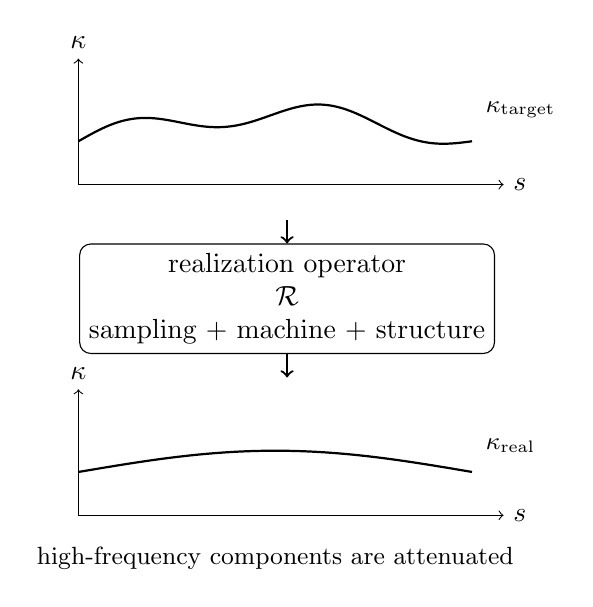
\begin{tikzpicture}[
  scale=1.0,
  axis/.style={->, thin},
  curve/.style={thick},
  label/.style={font=\small},
  box/.style={draw, rectangle, rounded corners, align=center, minimum width=3.2cm, minimum height=0.8cm}
]

\begin{scope}[shift={(0,3.0)}]
  \draw[axis] (0,0) -- (5.4,0) node[right] {$s$};
  \draw[axis] (0,0) -- (0,1.6) node[above] {$\kappa$};
  \draw[curve] plot[smooth, domain=0:5, samples=120]
    (\x,{0.55 + 0.35*sin(180*\x/5) + 0.14*sin(720*\x/5)});
  \node[label, right] at (5.05,0.95) {$\kappa_{\mathrm{target}}$};
\end{scope}

\node[box] (R) at (2.65,1.55) {realization operator \\ $\mathcal{R}$ \\ sampling + machine + structure};
\draw[->, thick] (2.65,2.55) -- (R.north);
\draw[->, thick] (R.south) -- (2.65,0.55);

\begin{scope}[shift={(0,-1.2)}]
  \draw[axis] (0,0) -- (5.4,0) node[right] {$s$};
  \draw[axis] (0,0) -- (0,1.6) node[above] {$\kappa$};
  \draw[curve] plot[smooth, domain=0:5, samples=120]
    (\x,{0.55 + 0.27*sin(180*\x/5)});
  \node[label, right] at (5.05,0.88) {$\kappa_{\mathrm{real}}$};
  \node[label] at (2.5,-0.55) {high-frequency components are attenuated};
\end{scope}

\end{tikzpicture}

\caption{Realization acts as a filtering process: target curvature may
contain high-frequency components that are attenuated by sampling,
machine action, and structural response.}
\label{fig:realization-filter}
\end{figure}

% ============================================================
\section{Realized Alignment}
% ============================================================

\begin{definition}[Realized alignment]
\label{def:realized-alignment}
The realized alignment is the physically constructed railway geometry,
denoted by
\[
\gamma_{\mathrm{real}}(s).
\]
\end{definition}

\begin{remark}
It may be represented continuously, but it is usually generated from
discrete construction, measurement, and maintenance data.
\end{remark}

\begin{definition}[Realized curvature]
\label{def:realized-curvature}
The realized curvature is:
\[
\kappa_{\mathrm{real}}(s)
=
\frac{\dd \theta_{\mathrm{real}}}{\dd s}.
\]
\end{definition}

\begin{remark}
The realized track should not be judged only by positional agreement,
but also by preservation of curvature evolution.
\end{remark}

% ============================================================
\section{Realization Error}
% ============================================================

\begin{definition}[Curvature realization error]
\label{def:curvature-realization-error}
A curvature-based realization error may be written as:
\[
\int_0^L
\bigl(\kappa_{\mathrm{real}}-\kappa_{\mathrm{target}}\bigr)^2
\,\dd s.
\]
\end{definition}

\begin{definition}[Curvature derivative error]
\label{def:curvature-derivative-error}
A higher-order realization error may be written as:
\[
\int_0^L
\bigl(\kappa'_{\mathrm{real}}-\kappa'_{\mathrm{target}}\bigr)^2
\,\dd s.
\]
\end{definition}

\begin{remark}
These measures reflect that different transition families may be close
in position space while differing significantly in curvature evolution
and dynamic interpretation.
\end{remark}

% ============================================================
\section{Sampling and Control Points}
% ============================================================

\begin{remark}
Construction and maintenance operate through discrete control data.
\end{remark}

\begin{definition}[Control points]
\label{def:control-points}
Let
\[
0=s_0 < s_1 < \dots < s_N = L
\]
be a strictly increasing sequence of arc-length positions.
These positions are called control points.
\end{definition}

\begin{remark}
The realized alignment may be reconstructed from these points using:
\begin{itemize}
\item piecewise linear interpolation,
\item piecewise polynomial interpolation,
\item spline-based reconstruction,
\item or machine-specific reconstruction rules.
\end{itemize}
\end{remark}

\begin{proposition}[Adaptive sampling principle]
\label{prop:adaptive-sampling-principle}
Sampling density should increase in regions of strong curvature
variation:
\[
\rho(s)
\sim
f\bigl(|\kappa'(s)|,|\kappa''(s)|\bigr),
\]
for a suitable increasing function \(f\).
\end{proposition}

\begin{remark}
Nearly constant-curvature regions require fewer control points, whereas
transition zones require denser control.
\end{remark}

% ============================================================
\section{Adjustment as Iterative Process}
% ============================================================

\begin{remark}
In railway construction and maintenance, track geometry is adjusted
through a sequence of localized operations, for example by tamping
machines.
\end{remark}

\begin{remark}
The canonical adjustment operator is denoted by \(\mathcal A\), as
introduced in \cref{def:adjustment-operator}.
\end{remark}

\begin{definition}[Iterative realization]
\label{def:iterative-construction-realization}
Starting from an initial alignment \(\gamma_0\), the iterative process is:
\[
\gamma_{k+1}
=
\mathcal A_{\gamma_{\mathrm{target}}}(\gamma_k).
\]
\end{definition}

\begin{remark}
The operator depends on local measurement data, machine parameters,
correction limits, and physical properties of the track.
\end{remark}

\begin{definition}[Realized alignment as limit]
\label{def:realized-alignment-limit}
If the sequence converges, the realized alignment is:
\[
\gamma_{\mathrm{real}}
=
\lim_{k\to\infty}\gamma_k.
\]
\end{definition}

\begin{proposition}[Fixed point interpretation]
\label{prop:realization-fixed-point}
If the iterative realization converges, then:
\[
\gamma_{\mathrm{real}}
=
\mathcal A_{\gamma_{\mathrm{target}}}(\gamma_{\mathrm{real}}).
\]
\end{proposition}

\begin{remark}
In practice, convergence cannot be assumed a priori, since it depends on
measurement feedback, machine limits, and local track conditions.
\end{remark}

% ============================================================
\section{Locality and Correction Limits}
% ============================================================

\begin{definition}[Local correction]
\label{def:local-correction}
A guided adjustment may be written as:
\[
\mathcal A_{\gamma_{\mathrm{target}}}(\gamma)
=
\gamma+\Delta(\gamma,\gamma_{\mathrm{target}}),
\]
where \(\Delta\) is a local correction operator.
\end{definition}

\begin{remark}
Typically, corrections are bounded:
\[
\|\Delta(\gamma,\gamma_{\mathrm{target}})\|
\le
\Delta_{\max}.
\]
\end{remark}

\begin{proposition}[Locality]
\label{prop:adjustment-locality}
The adjustment operator is local in the sense that:
\[
(\mathcal A_{\gamma_{\mathrm{target}}}\gamma)(s)
\]
depends only on \(\gamma\) and \(\gamma_{\mathrm{target}}\) in a
neighbourhood of \(s\).
\end{proposition}

\begin{remark}
This reflects the finite working range of construction and maintenance
equipment.
\end{remark}

% ============================================================
\section{Kernel-Based Realization Model}
% ============================================================

\begin{definition}[Kernel-based adjustment]
\label{def:kernel-based-adjustment}
A linearized model of the adjustment process is:
\[
(\mathcal A_{\gamma_{\mathrm{target}}}\gamma)(s)
=
\gamma(s)
+
\int_I
K(s,\sigma)
\bigl(
\gamma_{\mathrm{target}}(\sigma)-\gamma(\sigma)
\bigr)
\,\dd\sigma,
\]
where \(K(s,\sigma)\) is a localized influence kernel.
\end{definition}

\begin{remark}
The kernel represents the spatial influence of local construction or
maintenance action.
\end{remark}

\begin{proposition}[Localization]
\label{prop:kernel-localization}
There exists a characteristic length \(\ell>0\) such that:
\[
K(s,\sigma)\approx 0
\qquad
\text{for } |s-\sigma|>\ell.
\]
\end{proposition}

\begin{definition}[Discrete adjustment model]
\label{def:discrete-adjustment-model}
For control points \(s_i\), the kernel model becomes:
\[
\gamma_i^{(k+1)}
=
\gamma_i^{(k)}
+
\sum_j
K_{ij}
\bigl(
\gamma_j^{\mathrm{target}}-\gamma_j^{(k)}
\bigr).
\]
\end{definition}

\begin{remark}
This form is compatible with sparse numerical implementation.
\end{remark}

% ============================================================
\section{Filter Interpretation}
% ============================================================

\begin{proposition}
\label{prop:realization-low-pass}
The realization process acts approximately as a low-pass filter on
curvature.
\end{proposition}

\begin{remark}
High-frequency curvature components are attenuated during construction
and maintenance, while low-frequency structure is preserved.
\end{remark}

\begin{remark}
This explains why transition curves with similar low-order behaviour may
become nearly indistinguishable in position space after realization,
while still differing in curvature evolution and dynamic interpretation.
\end{remark}

% ============================================================
\section{Relation to the Realization Operator}
% ============================================================

\begin{remark}
In the AIM operator framework, realization is represented by:
\[
\mathcal R :
\mathcal X_{\mathrm{target}}
\rightarrow
\mathcal X_{\mathrm{real}},
\]
as introduced in \cref{def:realization-operator}.
\end{remark}

\begin{remark}
The construction process described in this chapter provides one
interpretation of how such an operator may arise physically.
\end{remark}

\begin{remark}
The simplified realization decomposition:
\[
\mathcal R
\approx
\mathcal M \circ \mathcal I \circ \mathcal S
\]
separates sampling, reconstruction, and mechanical response.
\end{remark}

% ============================================================
\section{Design Implication}
% ============================================================

\begin{remark}
The designed transition curve is not simply the curve that is built.
It is a target that produces a realized behaviour after construction and
maintenance.
\end{remark}

\begin{remark}
Thus, alignment design implicitly includes assumptions about
construction, machine behaviour, and structural response.
\end{remark}

\begin{proposition}
\label{prop:physical-design-space}
The relevant physical design space is the image of the realization
operator, not the full space of analytical curvature laws.
\end{proposition}

\begin{remark}
This connects construction and realization to realization-aware
optimization.
\end{remark}

% ============================================================
\section{Connection to AIM}
% ============================================================

\begin{summary}
Construction and realization describe the transformation from analytical
target alignment to physically realized railway geometry.

Within AIM, this transformation is treated as an explicit operator layer.

The realization layer explains why physical railway geometry must be
understood through construction processes, measurement feedback,
local correction limits, and mechanical response rather than through
analytical geometry alone.
\end{summary}
